\documentclass[10pt,journal]{IEEEtran}


\usepackage{amsfonts}
\usepackage{amsmath}
\usepackage{algorithm}
\usepackage{algorithmic}
\usepackage{amssymb}
\usepackage{graphicx}
\usepackage{cite}
\usepackage{subfigure}
\usepackage{float}
\usepackage{color}


\begin{document}


\title{DiDi Rescheduling}

\author{\IEEEauthorblockN{Feingming Zhu} \IEEEauthorblockN{Yucong Zhang} \IEEEauthorblockN{Weikai Xu} \IEEEauthorblockN{Ziqi Han} \IEEEauthorblockN{Ming Zhong}\\
\IEEEauthorblockA{School of Information Science and Technology\\
  ShanghaiTech University}} 
\maketitle

\begin{abstract}

This thesis explores a car rescheduling solution based on the data set provided by DiDi.
 
\end{abstract}


\section{Introduction}

Since the shared economy stepped into our life, it has been common to choose DiDi taxi as one of the means of the daily transportation. 
Therefore it is of great significance for DiDi to explore an efficient method to schedule the cars for the purpose of saving more time while making more income.\\

The main results and contributions of this report are summarized as follows:
\begin{itemize}
  \item \textbf{Initially modeling} 
  \item \textbf{Reframing}
  \item \textbf{Resolution and optimization}. 
  \item \textbf{Summary}.  
\end{itemize}


\section{Initially modeling}
\textbf{(i) Assumption}\\

Provided with datasets of the $GPS\ path$ and $order\ information$ of DiDi taxi in Chengdu on a certain day, we firstly come up with an idea about \textbf{clustering}, which can be illustrated in Fig.1. On such a heat map, the region in the big red circle can be designated as \textbf{busy} , while that in the yellow circle can be regarded as a \textbf{vacant} region. \\


\begin{figure}[!ht]
    \centering
    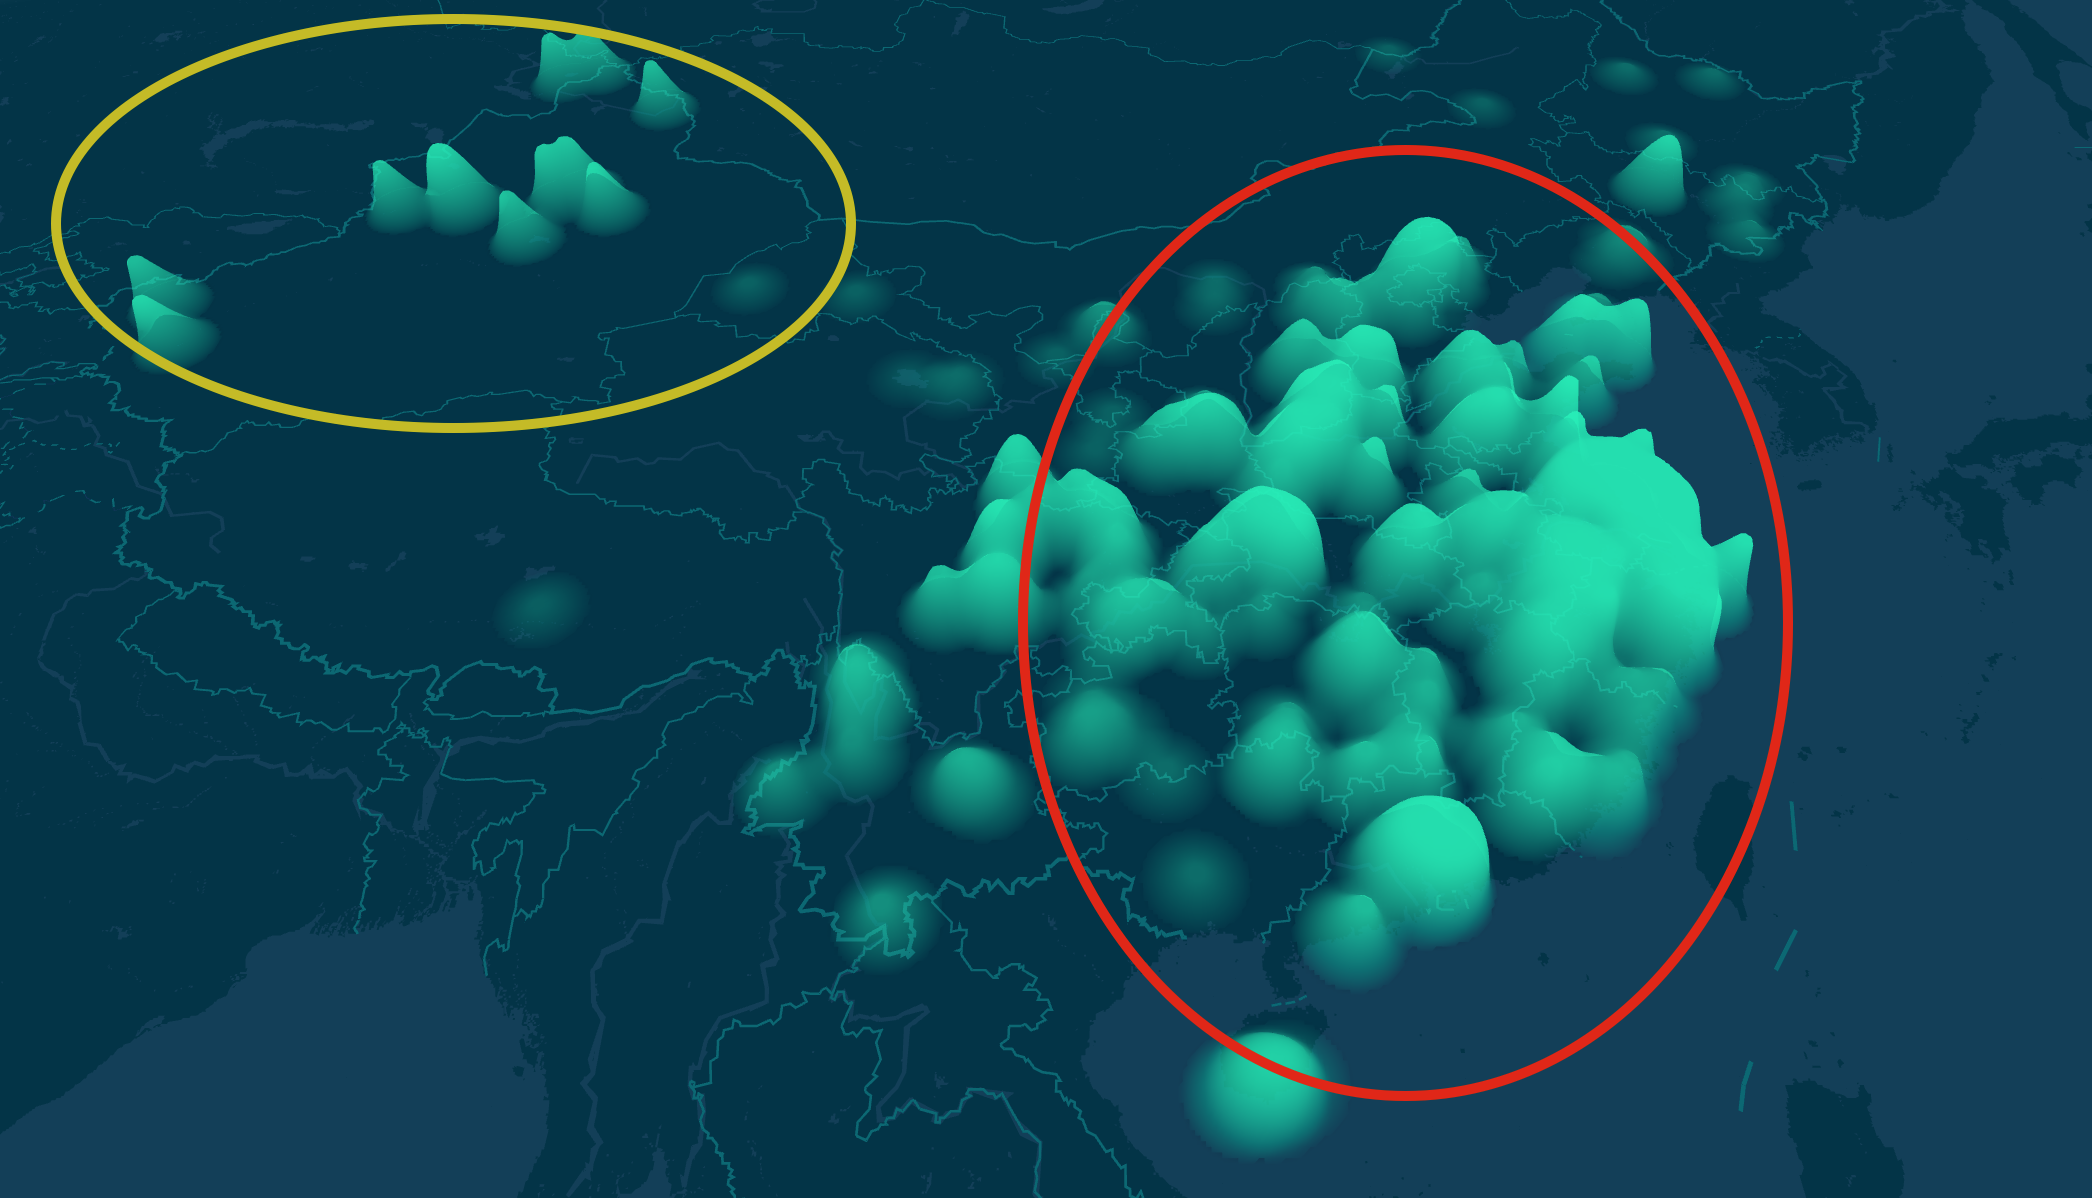
\includegraphics[width=0.9\columnwidth]{Fig/assumption.png}
    \caption{The assumed heat map}
 \end{figure}

In our assumption, if we plot the start point and the end point of each car in the $order\ dataset$ on the map, the heat distribution should be like Fig.1. Then, from the backend of DiDi, a message can be sent to the drivers in the red region, which may say, would you like to go to region yellow where cars may be needed? \\ 

\textbf{(ii) Data visualization}\\

After we plotting all the GPS points from $order\ dataset$, things are not going as we like. The visualization result is shown below.

\begin{figure}[!ht]
    \centering
    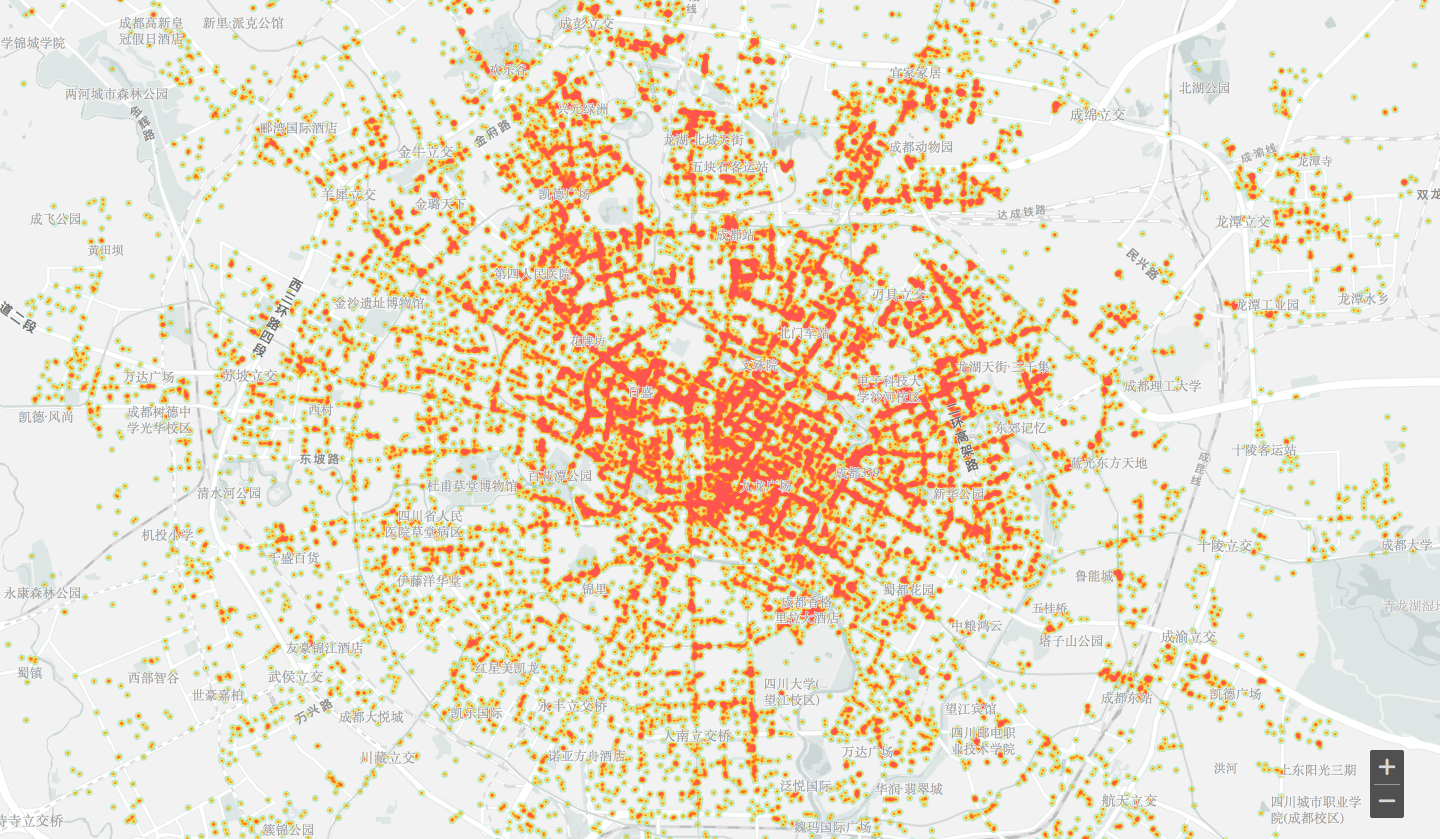
\includegraphics[width=1.0\columnwidth]{Fig/2D.png}
    \caption{The real heat map (2D)}
 \end{figure}

\begin{figure}[!ht]
    \centering
    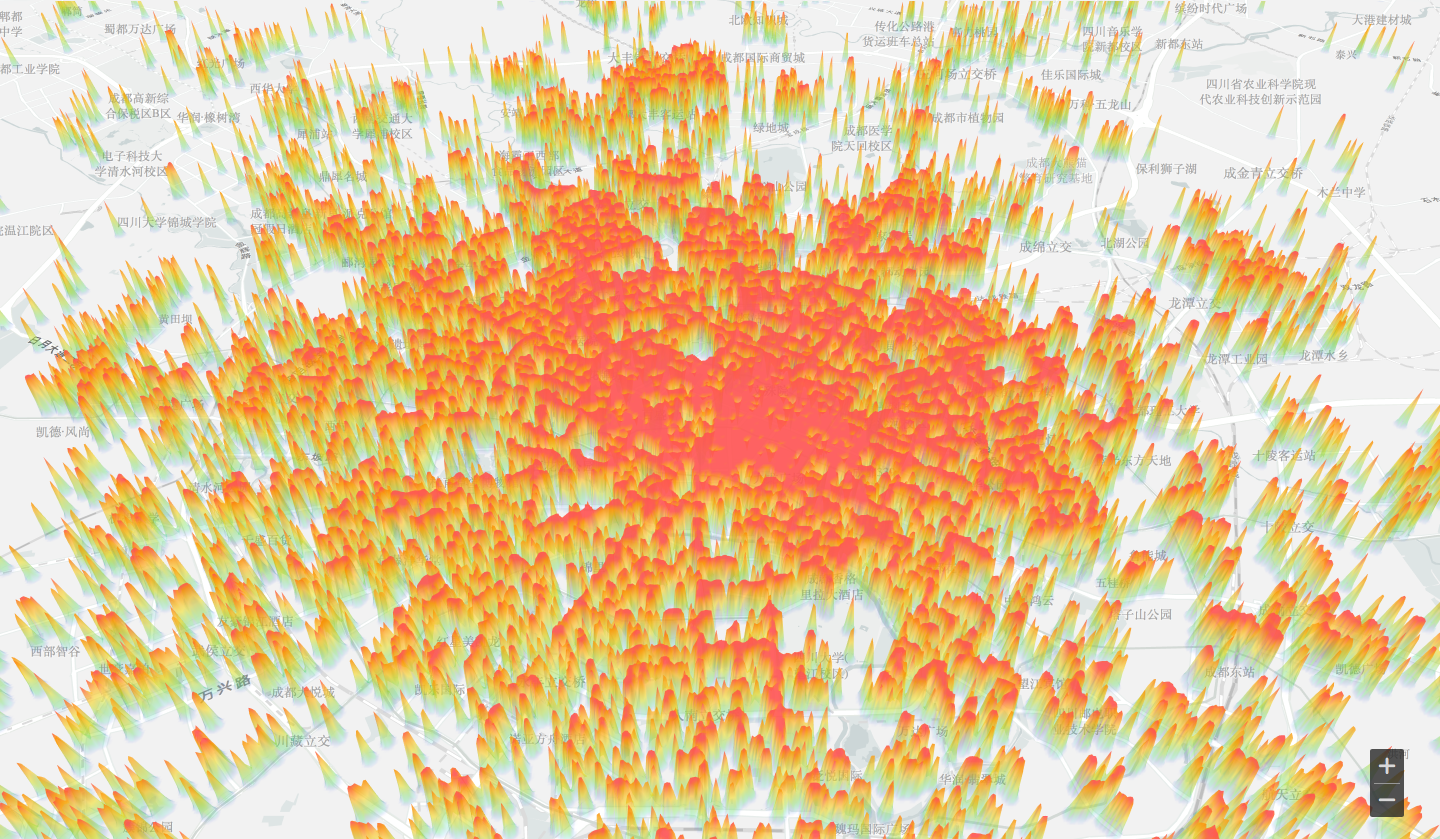
\includegraphics[width=1.0\columnwidth]{Fig/3D.png}
    \caption{The real heat map (3D)}
 \end{figure}

It is not much obvious that the gathered clusters scattered over the whole city, rather, the density of the center is reasonably high, but the radiation seems to be uniformly distributed. Therefore our previous assumption is \textbf{trivial} and \textbf{should be reframed}. \\
  
\section{Reframing}

\textbf{(i) Reframed assumption}\\

Although the previous assumption is really frustrating as it seems, it enlightens us to think about the regions. Since we cannot reach the conclusion that the $orders$ have some kind of tendency to cluster together, we reframed our assumption based on the views of those DiDi drivers, that is, what if it is not the density of orders but the preferred region of the drivers that matters.\\

\textbf{(ii) Visualization again}\\

Following this intuition, we then plot the $GPS\ route\ point$ for each driver to see what is going on with the $GPS$ $path$ $database$. For each driver, we set the $Driver\ ID$s as the control varieble. Then for each $Driver\ ID$, we record every $route\ point$ of every $Order\ ID$. Finally, the map with all the $route\ pointst$ of every driver should be able to generate the \textbf{active zones} of every single one of those drivers. Part of the processed data is shown below in Fig.4.

\begin{figure}[!ht]
    \centering
    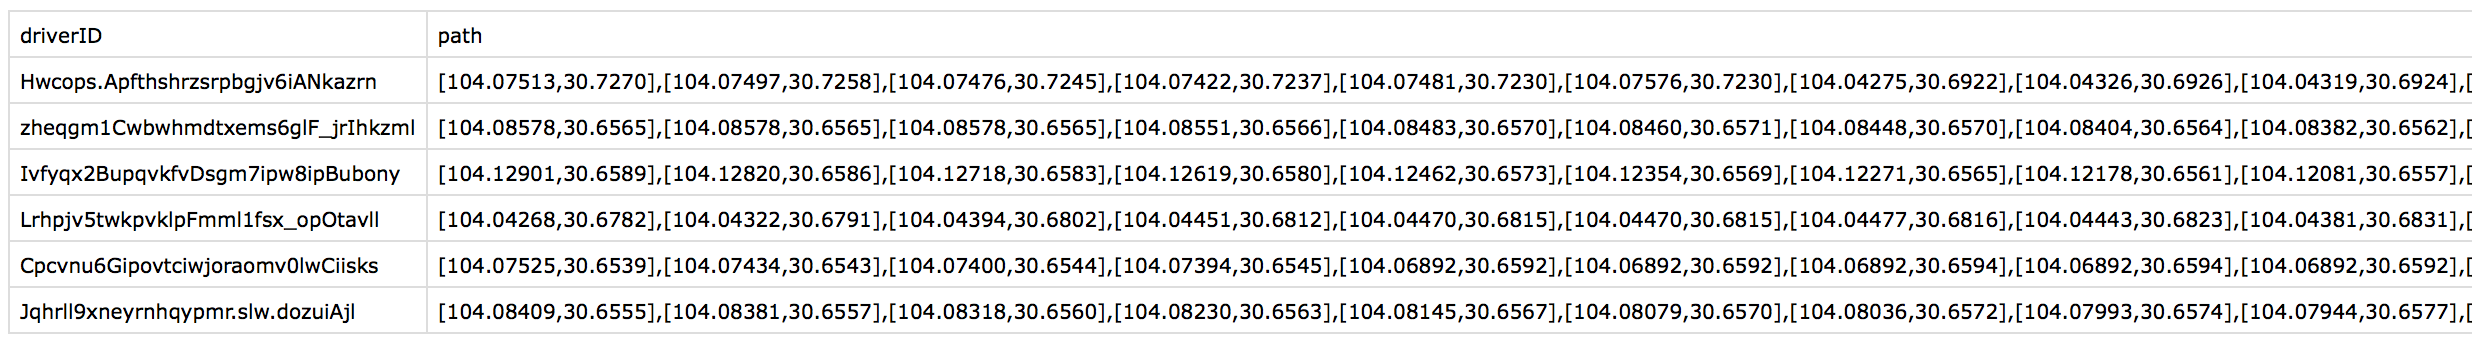
\includegraphics[width=0.9\columnwidth]{Fig/driverID.png}
    \caption{drivers with their route points}
 \end{figure}

\begin{figure}[!ht]
    \centering
    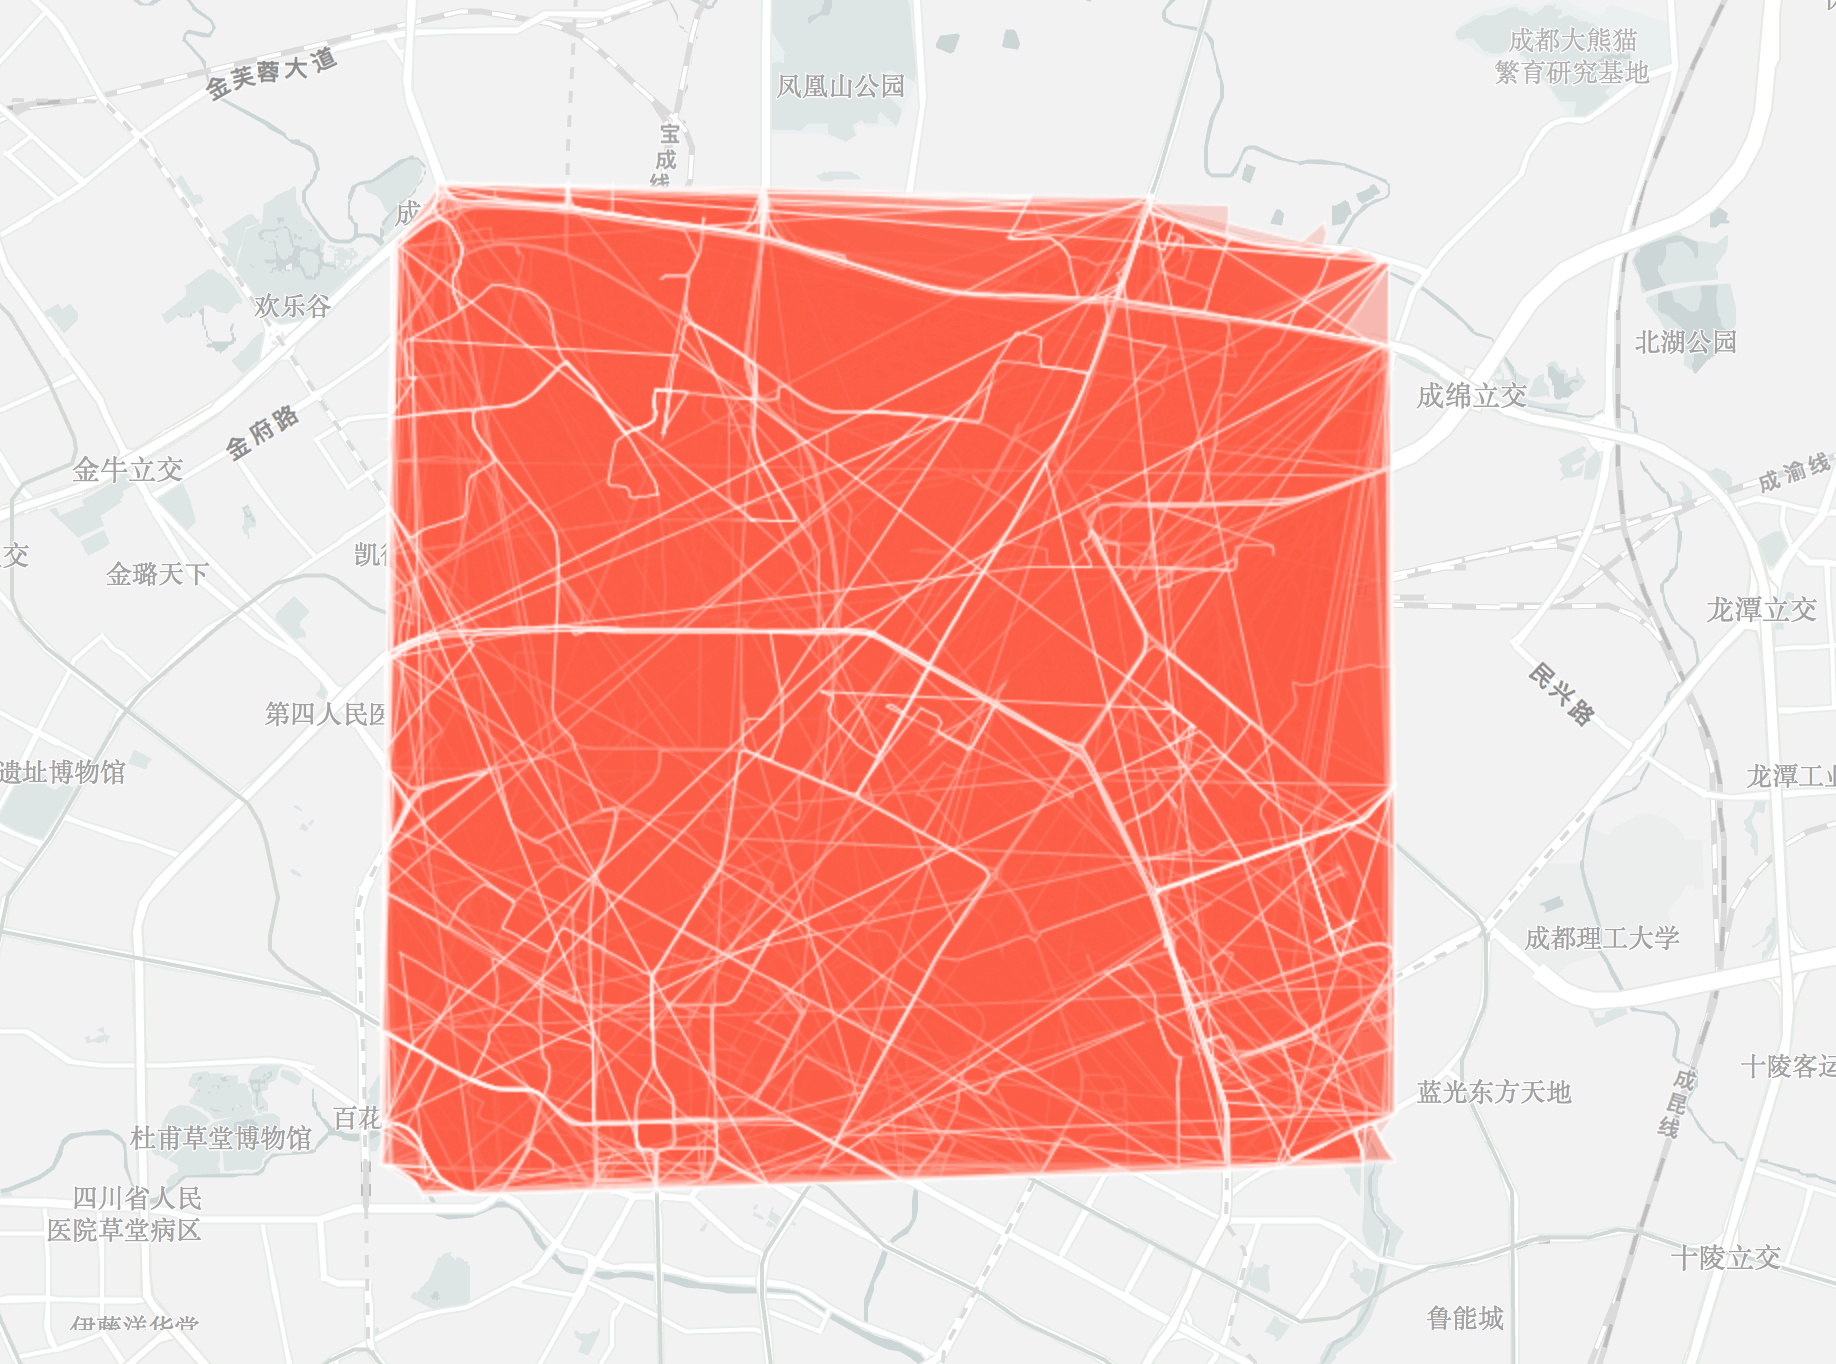
\includegraphics[width=0.8\columnwidth]{Fig/preferred_region_all.png}
    \caption{preferred regions of all the drivers}
 \end{figure}
 
 As we can see in Fig.5, it is totally a mess because the large database elicit a situation where all of those regions overlap and the API cannot provide us so many colors to clarify different preferred regions of different $Driver ID$s. To make it much more lucid, we choose 7 regions from it and recolor them as Fig.6 below.
 
 \begin{figure}[!ht]
    \centering
    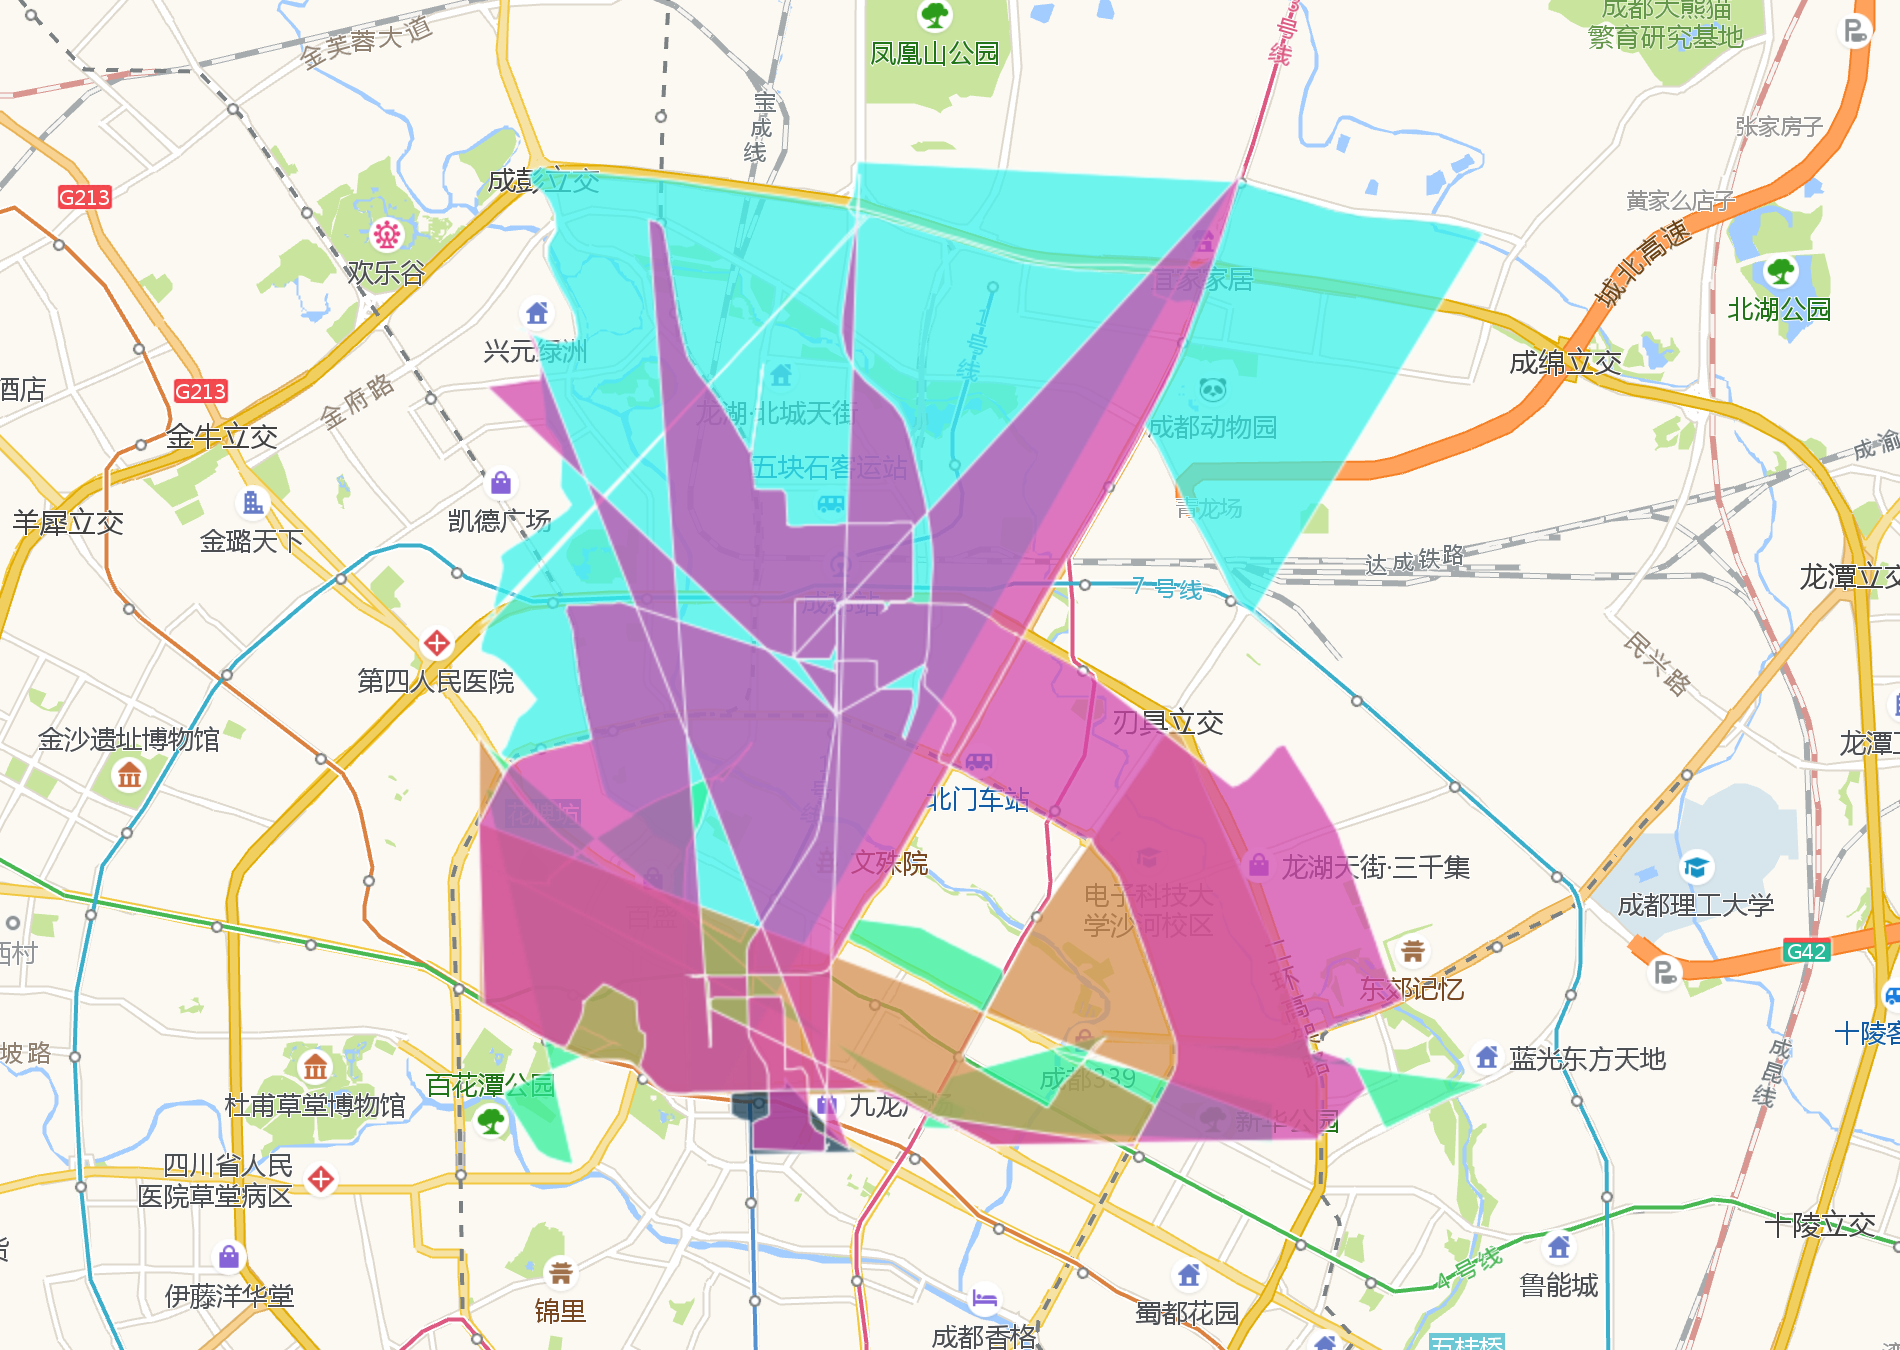
\includegraphics[width=0.7\columnwidth]{Fig/preferred_region_7.png}
    \caption{preferred regions of 7 drivers}
 \end{figure}
 

Fig.6 above shows that different drivers indeed have different routes. We may basically attribute the fact that the active zone differs from driver to driver to several reasons, their homes, their familiarity of the region, etc. From the view of the customers, we simply want to get to the location comfortably and especially quickly. Hence, the familiarity of the regions is quite important. Since those regions are both familiar and the active zones of those drivers, we simply defined those colored regions as \textbf{preferred regions} for each driver.

 
 \begin{figure}[!ht]
    \centering
    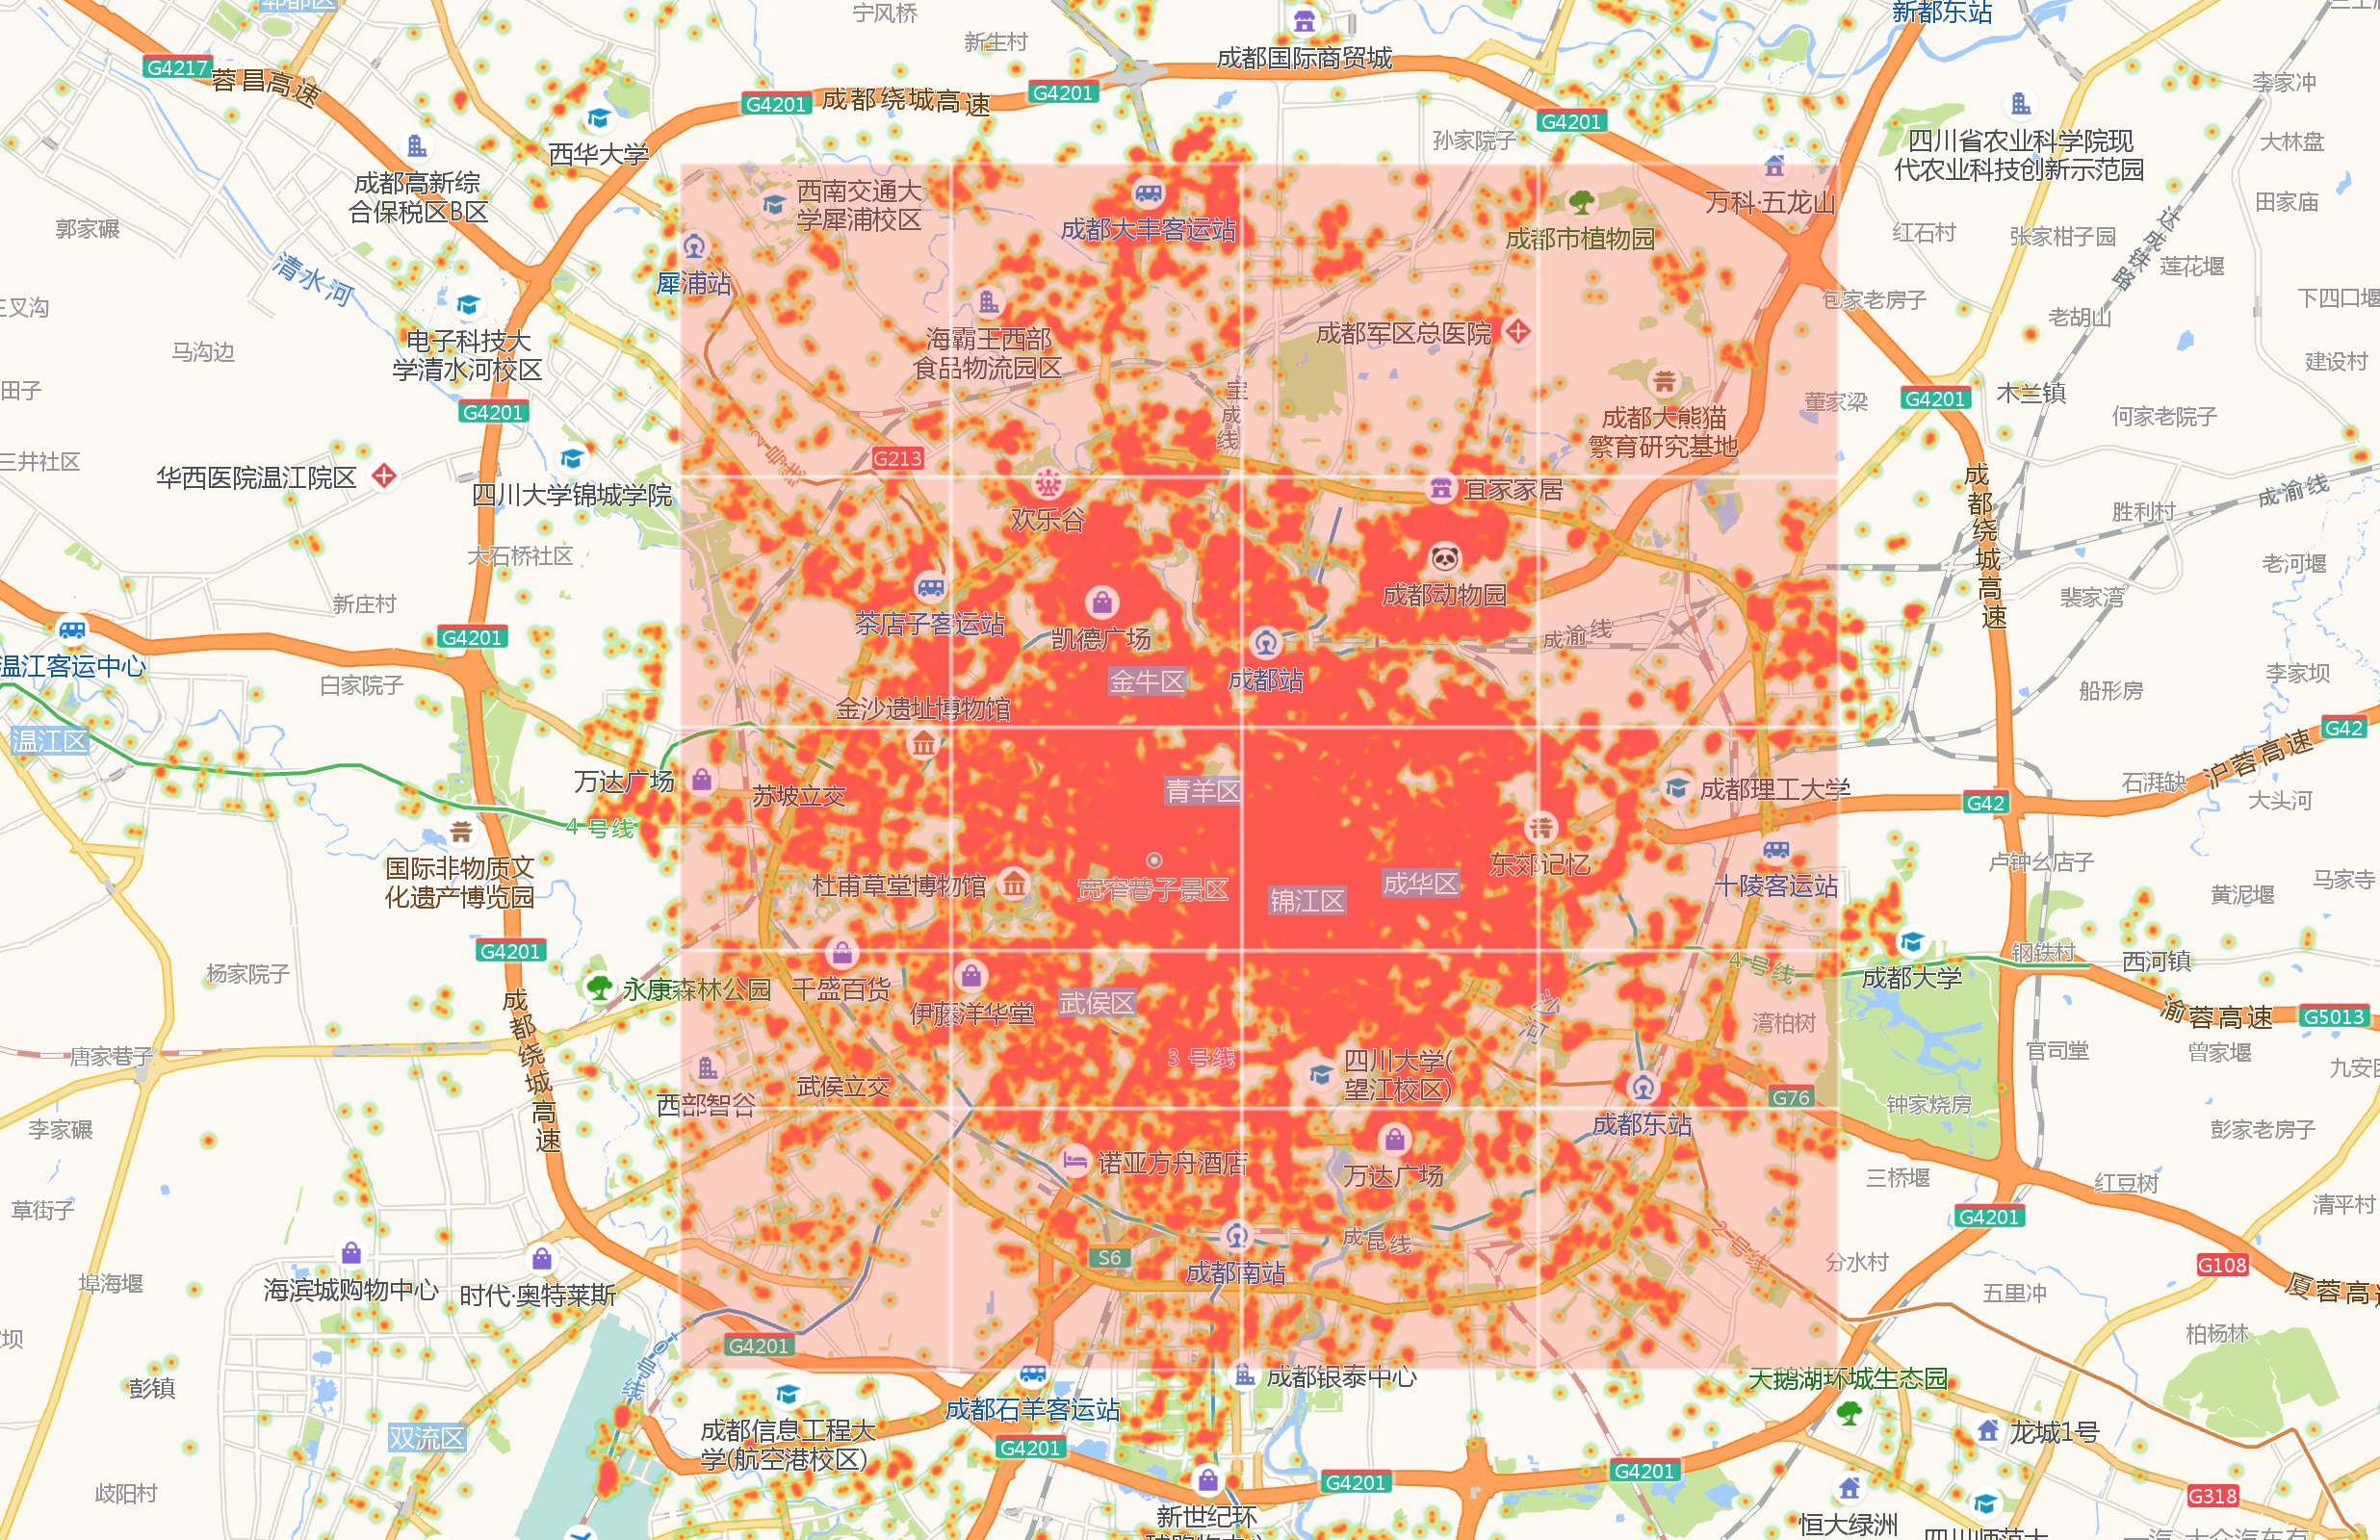
\includegraphics[width=1.0\columnwidth]{Fig/region.png}
    \caption{heat map with a rectangle}
 \end{figure}
 
 Back to the previous heat map(Fig.2), we roughly overlay a rectangle onto it to make most of the heat points inside (we choose a rectangle rather a circle to make the prototype model simple), as illustrated in Fig.7. The big rectangle is divided into $5*4$ sub-rectangles. And when Fig.6 and Fig.7 are combined together, as Fig.8, it can be found that one single driver' \textbf{preferred region} intersect with one or several sub-rectangles. For example, the blue \textbf{preferred region} mainly intersects sub-rectangles in (2,2), (2,3), (3,2).

 \begin{figure}[!ht]
    \centering
    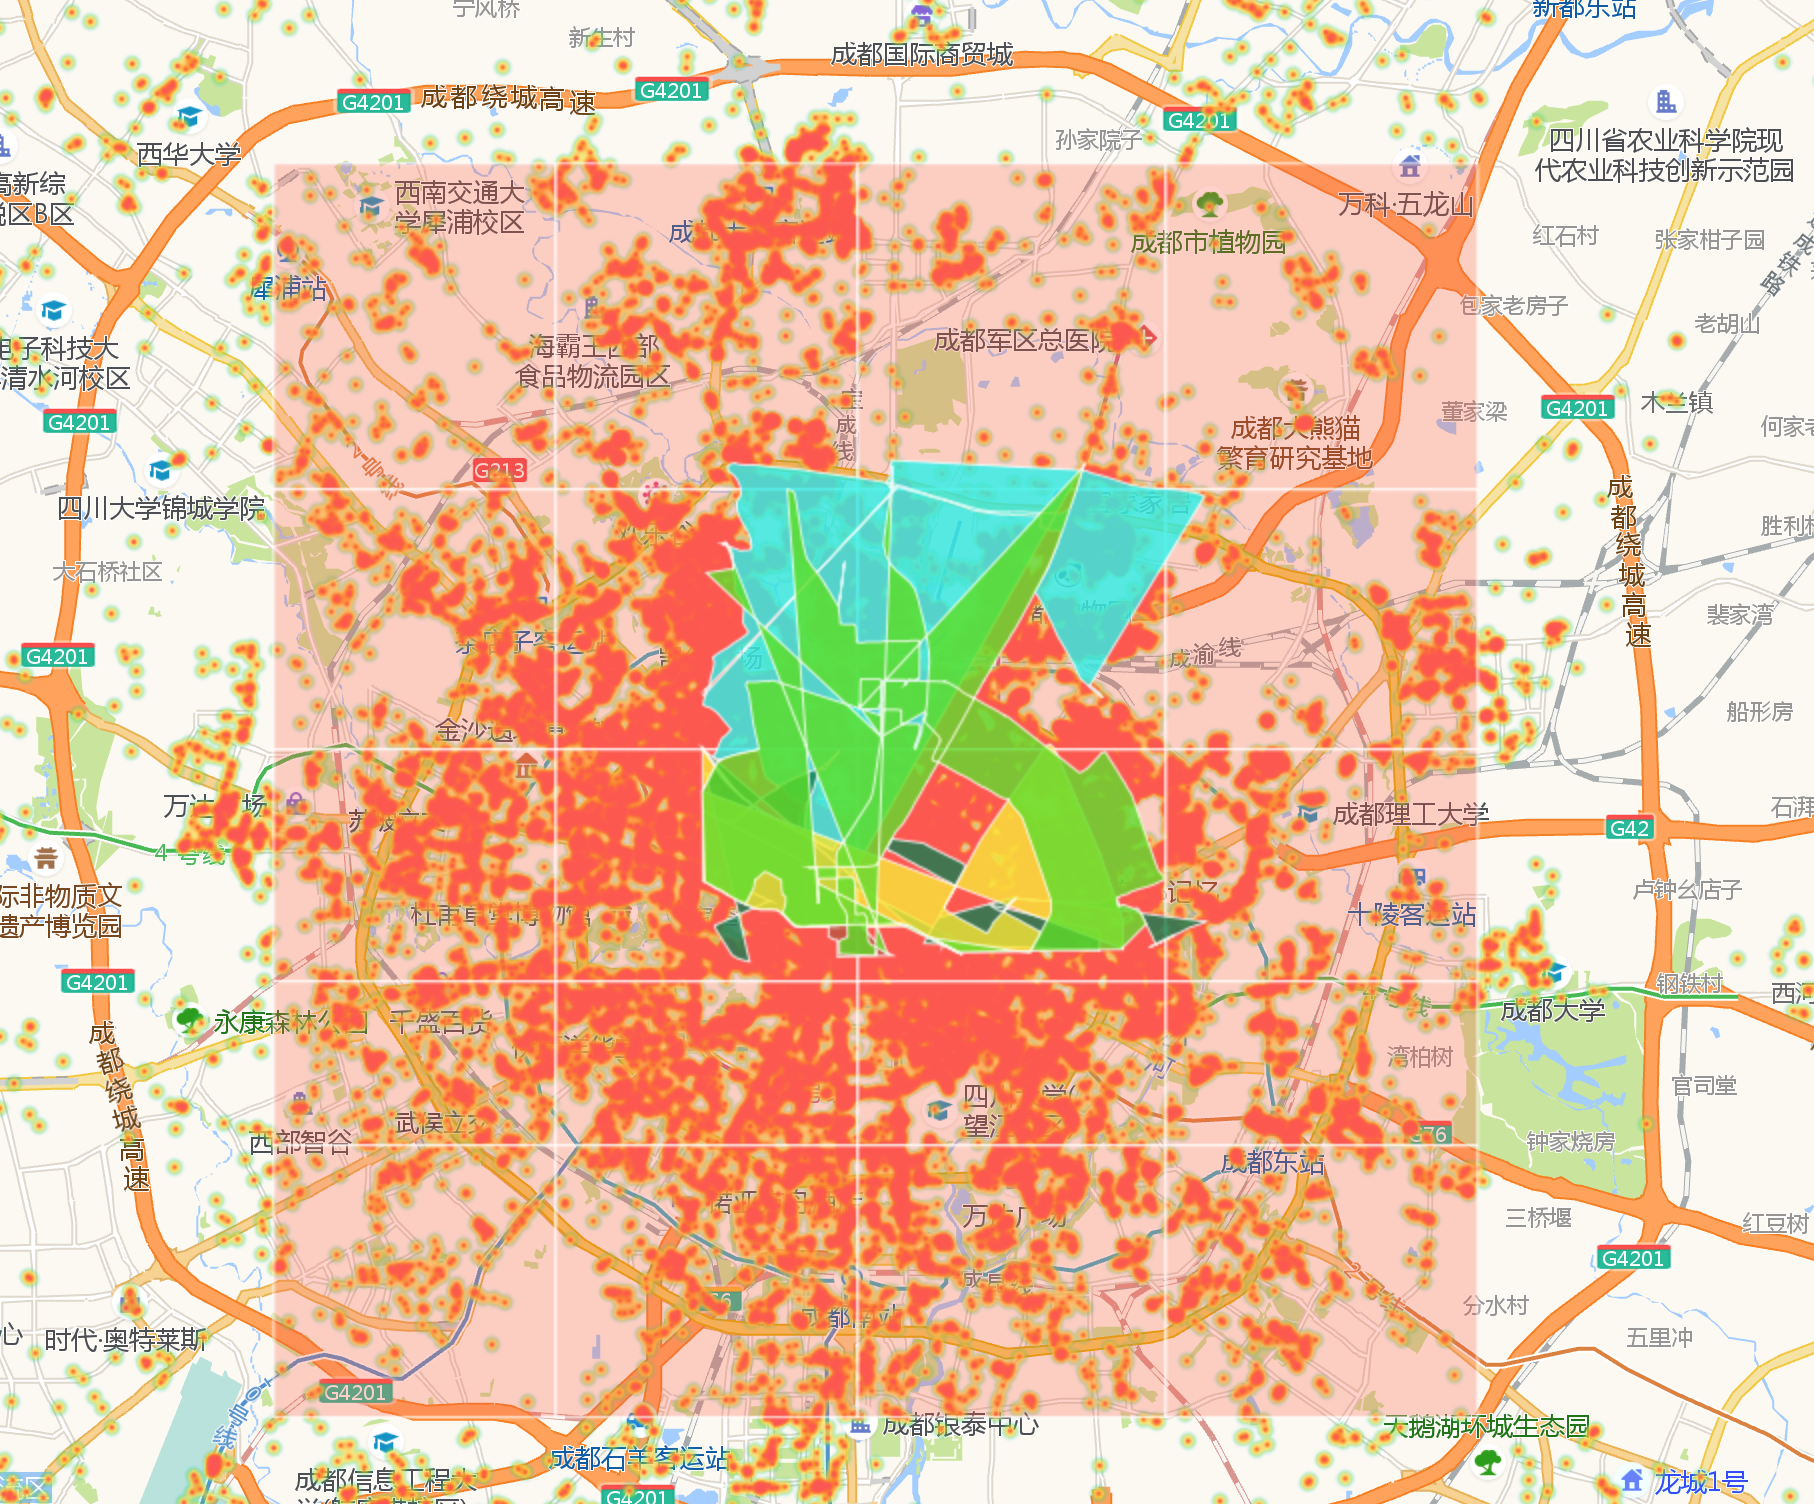
\includegraphics[width=1.0\columnwidth]{Fig/preferred_region_with_heat.png}
    \caption{preferred regions of 7 drivers plus the heat map and the rectangle}
 \end{figure}



\section{Resolution and Optimization}

\textbf{(i) Algorithm}\\

According to Fig.8, the numbers of cars in each sub-rectangle can be obtained, which can be regarded as the \textbf{historical number of needed cars}.  
Suppose we can acquire the \textbf{real-time number of cars} in each sub-rectangle, then we can know whether the sub-rectangle needs the car or has more cars. \\

We implement two priority queues. \textbf{Priority queue I} is for the sub-rectangles which need cars and \textbf{Priority queue II} is for the sub-rectangles which have more cars. Then we decide each sub-rectangle belongs to which priority queue, and insert it into one of these two priority queue.\\

Every ten seconds, we pop the sub-rectangle with the highest priority. Firstly, it should be determined whether these two sub-rectangles are far. If so, we pop one more sub-rectangle from \textbf{ priority queue II} and push the first popped sub-rectangle from \textbf{priority queue II} back to it. Such a loop lasts until 2 close enough(may need a threshold here) sub-rectangles are found.\\

 The sub-rectangle from  \textbf{Priority queue I} is designated as \textbf{target}, while that from \textbf{Priority queue II} is designated as \textbf{source}. The next step is to find all the cars in the \textbf{source}, if there is a car whose driver's \textbf{preferred region} intersects with \textbf{target}, a message will be sent to notify the driver, which may say, would you like to go to xxx, you may get more orders there. \underline{\textbf{ The control flow is shown in Fig.9.}}\\
 
 \begin{figure}[!ht]
    \centering
    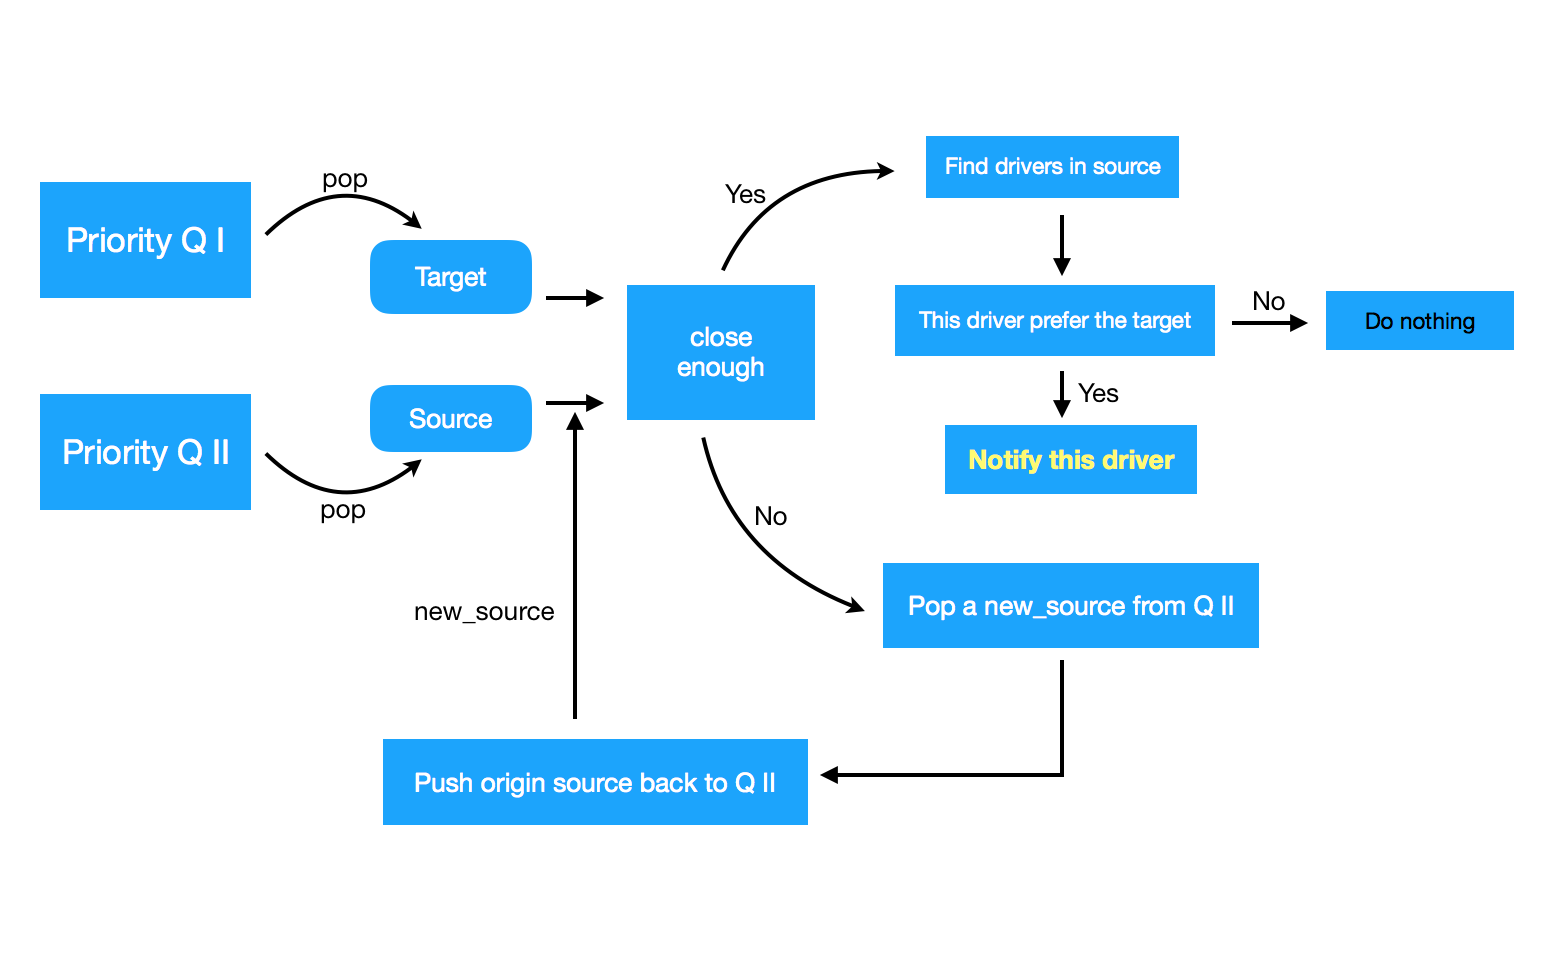
\includegraphics[width=1.0\columnwidth]{Fig/control_flow.png}
    \caption{the car object implementation}
 \end{figure}

And after that, we update these two priority queues.\\

\textbf{(ii) Implementation}\\

As for the implementation, the 2 main Objects are shown below in Fig.10 and Fig.11. It should be noted that what we call sub-rectangle is implemented as \textbf{class Region} for the further generalization.
 \begin{figure}[!ht]
    \centering
    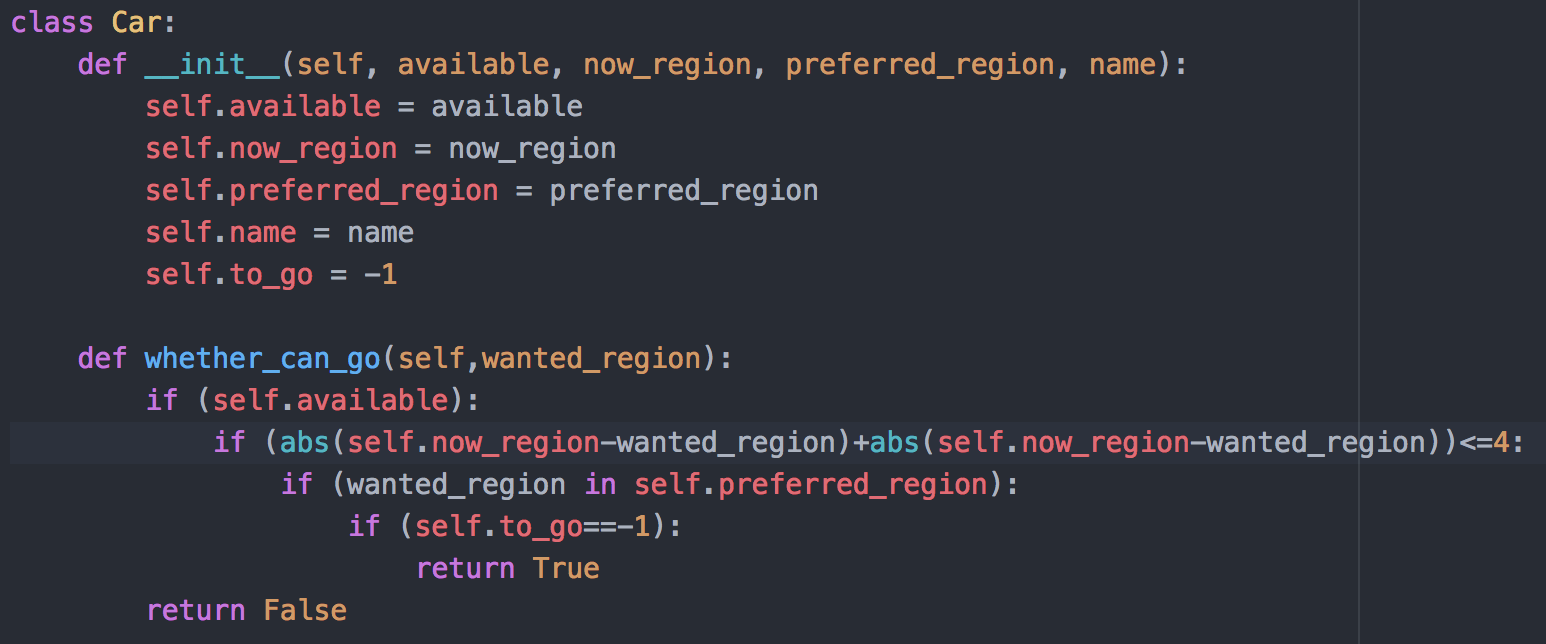
\includegraphics[width=1.0\columnwidth]{Fig/class_car.png}
    \caption{the car object implementation}
 \end{figure}

 \begin{figure}[!ht]
    \centering
    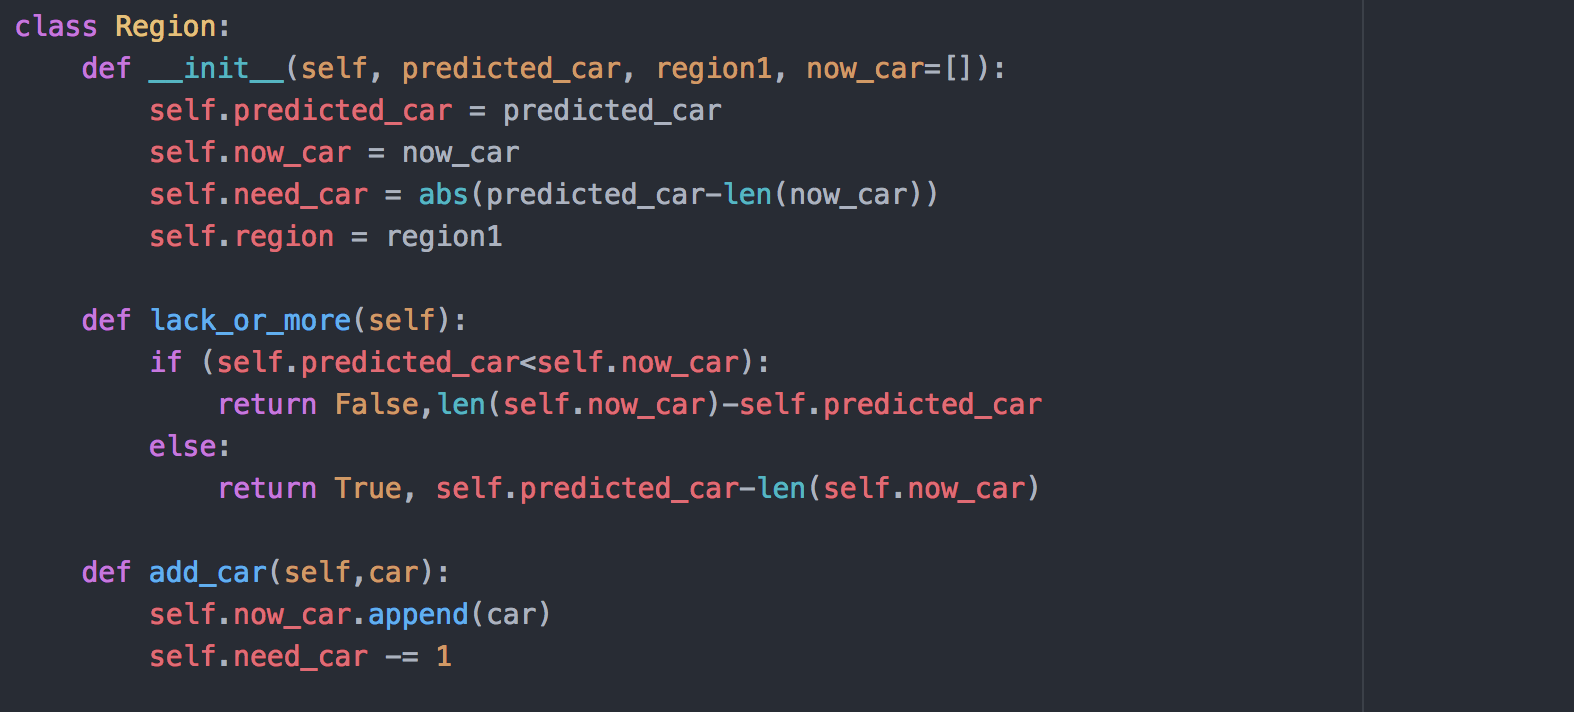
\includegraphics[width=1.0\columnwidth]{Fig/class_region.png}
    \caption{the region object implementation}
 \end{figure}



\section{Summary}

\textbf{(i) Conclusion}\\

 Through our optimized resolution, the scheduling of DiDi cars can be somehow more balanced. The goal of making more income while saving more time is primarily achieved.\\
 
 \textbf{(ii) Some Flaws}\\
\begin{itemize}
  \item In previous part, we adopted rectangles as divided regions, which lacks generalization.  
  \item The execution of our algorithm consists of obtaining and processing the real-time data, which may cost a giant time complexity. 
\end{itemize}

 
%\pagebreak
\section*{Acknowledgment}
During this project, we collaborated and discussed within a group of classmates Fengming Zhu, Yucong Zhang, Weikai Xu, Ziqi Han and Ming Zhong. The data is from DiDi. We also refer to some contents from Gaode API\cite{Gaode}.  



\bibliographystyle{IEEEtran}
\bibliography{Reference}






\end{document}


